%! Author = raquelmolire
%! Date = 25/09/2022

El alzheimer es una enfermedad neurodegenerativa, progresiva, irreversible y terminal en la que se produce una pérdida
de neuronas principalmente relacionada con dos tipos de alteraciones cerebrales: la acumulación anormal de placas
seniles de proteína beta-amiloide y ovillos neurofibrilares de proteína Tau.

\subsection{Epidemiología de la enfermedad}\label{subsec:epidemiologia}
Es la forma más común de demencia, una pérdida de la función cerebral que afecta la memoria, el pensamiento, el
lenguaje, el juicio y el comportamiento.
Se estima que entre un 60 y un 80 por ciento de los casos de demencia se producen a causa de la EA en los países
desarrollados.

Esta patología tiene una mayor frecuencia en personas mayores de 65 años, siendo la prevalencia de un 7\% en este grupo
de población, y aproximándose al 50\% en mayores de 85 años.
Aunque en otros casos más extremos y mucho menos frecuentes puede ser desarrollada a partir de los 30 años, siendo
denominada en este caso como Enfermedad de Alzheimer precoz o de aparición temprana.
En término medio, una persona con Alzheimer vive de 4 a 8 años después de ser diagnosticada, pero puede vivir hasta 20
años dependiendo de otros factores como es, por ejemplo, la etapa en la que se diagnostique la enfermedad.

Actualmente, en España la cifra de personas afectadas por la enfermedad del Alzheimer es de aproximadamente 1.200.000,
aproximándose a las 5.000.000 personas si contamos con la familia.

\subsection{Cuadro clínico}\label{subsec:cuadro-clinico}
Las lesiones cerebrales características de la EA comienzan años antes de que aparezcan los primeros síntomas, según
concluyen algunas investigaciones, estas alteraciones cerebrales pueden darse entre 10 o 20 años antes.

La EA produce en el cerebro una pérdida neuronal progresiva que se relaciona de manera directa con la acumulación de
placas de proteína beta-amiloide y de ovillos neurofibrilares de proteína Tau que impiden a las neuronas comunicarse
entre sí conduciendo a su muerte.
El conjunto de estas lesiones se inicia en el hipocampo y se distribuye a otras regiones cerebrales según el grado de
evolución de la enfermedad.

El hipocampo es una de las áreas del cerebro cuyo funcionamiento es vital para la memoria y el aprendizaje.
Este es el motivo por el cual, en las primeras etapas de la enfermedad, las personas con EA presentan dificultades para
recordar sucesos recientes o para retener información nueva, sin embargo, se conservan recuerdos del pasado porque las
zonas del cerebro implicadas todavía no se han visto afectadas.

La afectación progresiva de otras áreas cerebrales da lugar a la aparición de otros síntomas que afectan a la toma de
decisiones, cambios conductuales y de personalidad, dificultad para la comunicación y la pérdida de funciones biológicas
que conlleva la muerte.

El desarrollo progresivo de la EA es lo que da lugar a que se establezca una distinción de etapas de la enfermedad según
la evolución de las lesiones en el cerebro y según la evolución de los síntomas que van produciendo esos daños.
Distinguiendo tres etapas: enfermedad de Alzheimer leve (etapa temprana), enfermedad de Alzheimer moderada (etapa media)
y enfermedad de Alzheimer grave (etapa final), las cuales se detallan posteriormente.

\subsection{Cómo afecta al funcionamiento cerebral la acumulación de proteína beta-amiloide y Tau}\label{subsec:
acumulacion-proteínas}
La acumulación en el cerebro de placas de proteína beta-amiloide y de ovillos neurofibrilares de proteína Tau provoca la
interrupción de la comunicación, el metabolismo y la reparación de neuronas, que son los procesos que hacen que las
neuronas se mantengan sanas.
La suspensión de estos procesos provoca la muerte de neuronas, y es la que conlleva problemas de memoria.

La proteína beta-amiloide es una proteína presente en el cerebro que lleva a cabo determinadas funciones fisiológicas.
En una persona con EA, la eliminación de los restos de esta proteína no se realiza de manera correcta, provocando la
formación de placas seniles (depósitos extracelulares de beta-amiloide) y afectando al funcionamiento cerebral normal.


La proteína Tau tiene como principal objetivo mantener la estructura de las neuronas.
En personas con EA, se provoca una serie de alteraciones bioquímicas que causan la formación de ovillos neurofibrilares
como un conglomerado anormal de proteínas que se compone de pequeñas fibrillas entrelazadas en el interior de las
neuronas.

A medida que las neuronas mueren y las conexiones entre las redes de neuronas se rompen, muchas regiones del cerebro
comienzan a encogerse.
En la etapa final de la EA, el daño cerebral producido es muy grande, resultando una pérdida significativa del volumen
de tejido cerebral.

\begin{figure}[H]
    \centering
    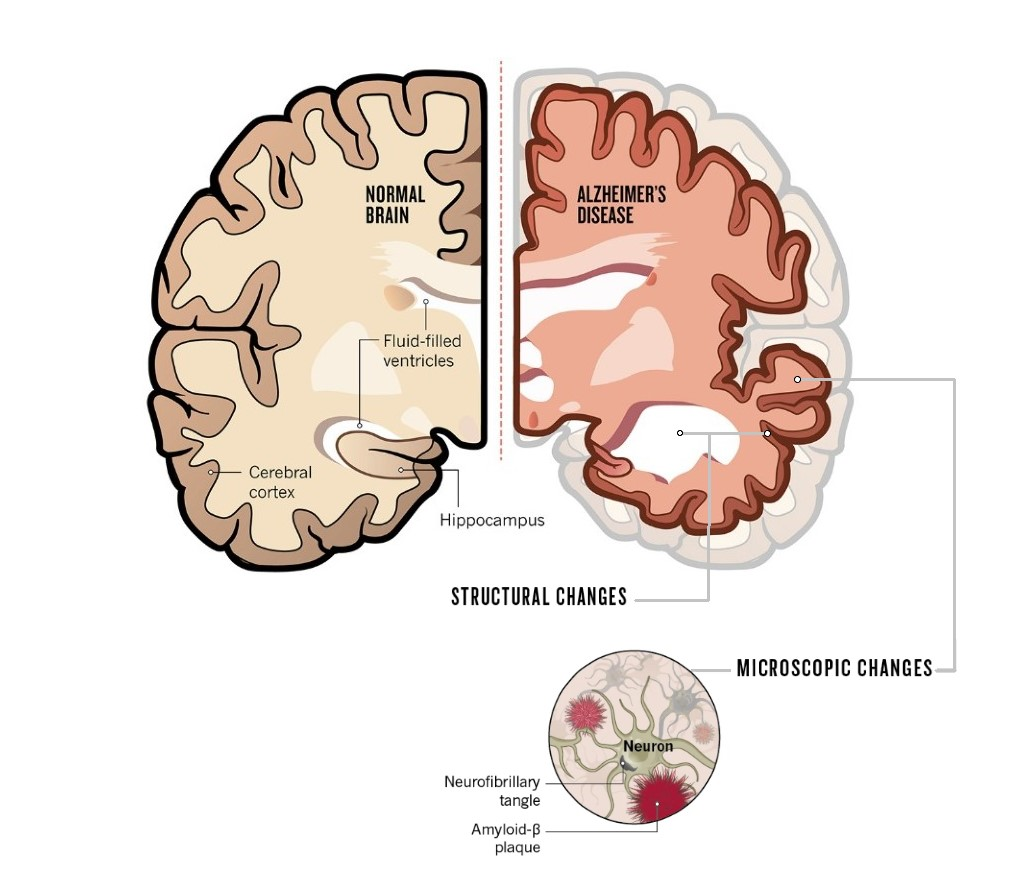
\includegraphics[width=\textwidth]{./imgs/lesiones-cerebrales}
    \caption{Lesiones cerebrales producidas por la enfermedad de Alzheimer.\\Imágen adaptada de una
    ilustración de Stacy Jannis, Alzheimer\'s Association.}
    \label{fig:lesiones-cerebrales}
\end{figure}


